\begin{center}
 \begin{minipage}[b]{0.45\textwidth} 
\subsection*{General information}
Name: David Rasmussen \\
Address: Islands brygge 56b 1tv \\
Zip nr. 2300 Koebenhavn S \\
Phone number: 26325635 \\
E-mail: david2300@hotmail.com \\
Country: Danmark \\
Date of birth: 11/06/1995
\newline
 \end{minipage}
 \hfill
\begin{minipage}[b]{4.5cm}
 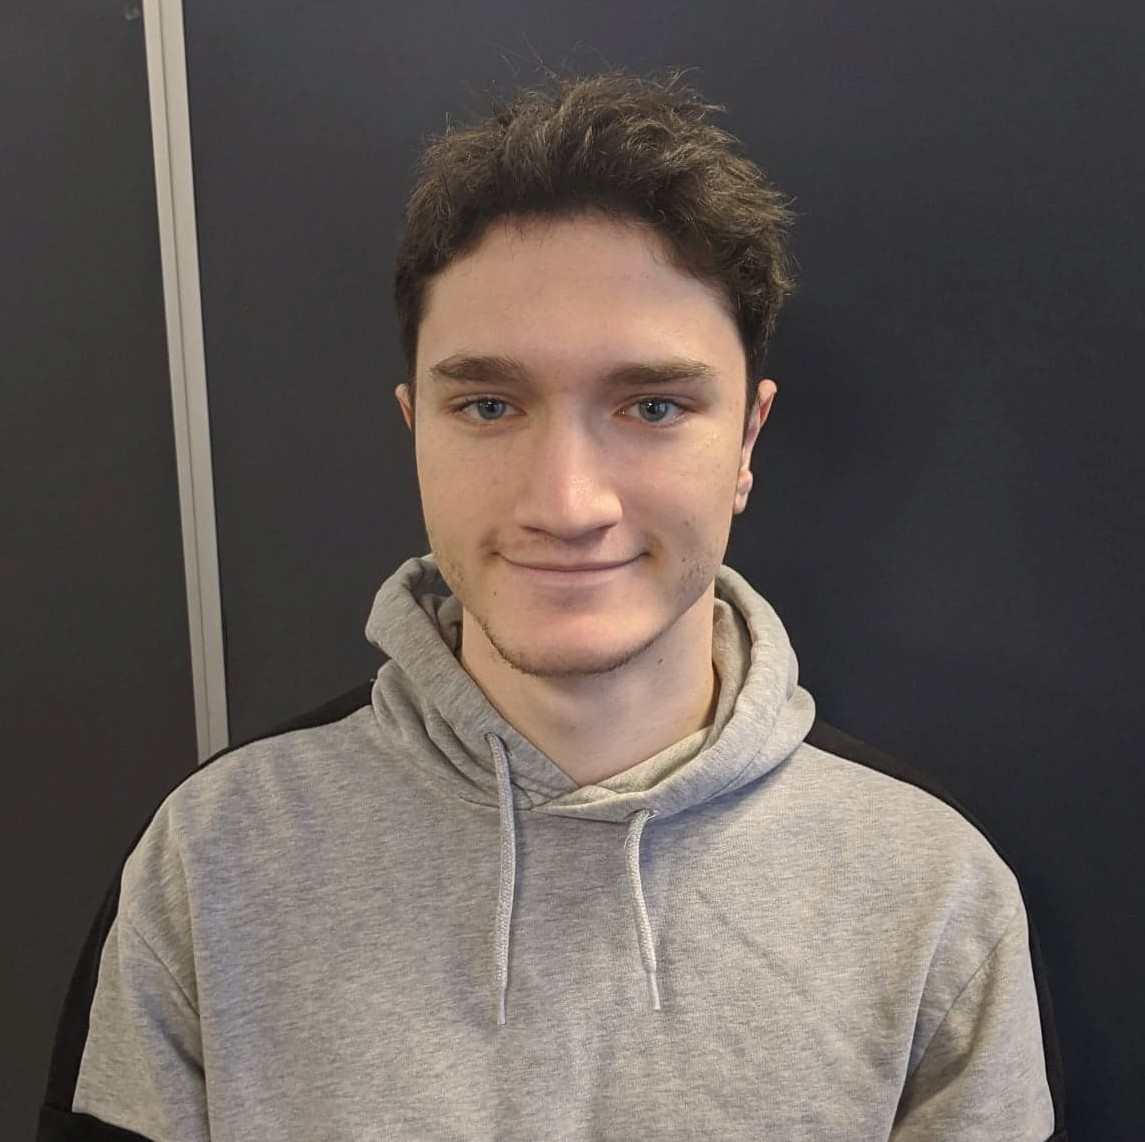
\includegraphics[height=4.25cm]{figures/Billede_af_David}
 \end{minipage}
 \end{center}

\section*{Work experience}
\begin{itemize}
\item 2010 - 2012 Netto - Sevice employee
\item 2012 - 2013 Bauhaus Valby - Salesman
\item 2013 - 2014 Q8 - Sales Assistant
\item 2016 - 2018 Elgiganten Glostrup - Cross operation 
\item 2018 - 2020 Concept - Client service 
\end{itemize}
\section*{Education}
\begin{itemize}
\item 2011 - 2014 HTX-Hilleroed, Biotech
\item 2015 - 2018 Aalborg university Bachelor of Software Engineering
\item 2018 - 2020 Aalborg university Master of Software Engineering
\end{itemize}

\section*{Background Information}
Learned to tackle multiple things at once, while working at Q8, since I was alone in the shop.\\Was responsible for handling company customers at Bauhaus.\\Slogan is "if its worth doing, then its worth doing properly".\\Everything I do, I try to be a perfectionist about it.\\Fluent in english and danish.\\Highschool exam project was using c sharp (unity) to make a game.\\Elementary understand of business and economics.\\Taken courses in analysis.\\Incredibly disciplined, and work good in teams.\\Lots of skills in programming.\\Good fundamental understanding of databases.\\Large interest in electronics. Done multiple projects.\\Through university, I have learned c in depth.\\Proficient in C++.\\Made my own website using Javascript, HTML5 and CSS.\\Able to do mathematical optimization using matlab.\\Earlier work include: working at a sushi restaurant, Bilka, bauhaus, Q8, and with selling christmas trees. Because of this, im disciplined in customer service.\\Also good at handling lots of things at once, without getting stressed out. Took a high school diploma in biotechnology: finished with a grade of 10.7.\\Throughout highschool, I joined a lot of extra curricala activities.\\Love presenting: therefore heavily improved my oral skills.\\Of my core interests lie in history.\\Love discussion philosophy, and especially moral ambiguities.\\Read a lot of philosophy in my free time.\\Concise and well spoken in my communication.\\Was an incredible dedicated person.\\Done multiple extra projects in my free time.\\Made my own self driving RC car.\\Made a robot, that can drive on its own.\\Spent a lot of time during integrated circuits in my free time.\\Once made an embedded electronic watch/thermometer for my girlfriend.\\Love helping people.\\Taken a BSc and MSc degree in software engineering.\\Bsc was focused on group work, which has honned my team skills.\\Was always the teamleader during group projects.\\Did a multi group project, which made me good at agile and large scale software development.\\Experience using Git as a resource management tool.\\Specialized in articifial intelligence and cloud computing.\\Expertise in javascript, .Net, Css, Html, SQL to do general web programming.\\Experience in python using their libraries to do machine learning.\\Good experience using Java\\done a lot of lowlevel programming, including: microproccessor programming, and using the language C.\\
